\documentclass[a4paper, 10pt]{article}
\hyphenpenalty=8000
\textwidth=125mm
\textheight=185mm

\usepackage{graphicx}
%this package is flexible for image insertion
%
\usepackage{alltt}
%this package is suitable for the description of algorithms and computer programs
%
\usepackage{amsmath}
%this package draws mathematical symbols smoothly
%
\usepackage[hidelinks, pdftex]{hyperref}
%this package produces hypertext links in the document

\pagenumbering{arabic}
\setcounter{page}{1}
\renewcommand{\thefootnote}{\fnsymbol{footnote}}
\newcommand{\doi}[1]{\href{https://doi.org/#1}{\texttt{https://doi.org/#1}}}

\begin{document}

\begin{center}
Nonlinear Analysis: Modelling and Control, Vol. vv, No. nn, 2025\05\03
\copyright\ IE Infotep\\[24pt]
\LARGE
\textbf{Analisis Univariado y Multivariado}\footnote{This research was supported by grant No.\ xxxx.}\\[6pt]
\small
\textbf {Aris Avila, Julieth Gutierrez, Diego Alzate}\\[6pt]
\end{center}

\begin{abstract}
Este estudio analiza los datos de viviendas en California, explorando la relación entre variables clave como el valor mediano de la vivienda, el número total de habitaciones y el número total de dormitorios. Se realizan análisis univariados y multivariados para identificar patrones y correlaciones, utilizando visualizaciones como histogramas, diagramas de caja y gráficos de dispersión. Los resultados indican que ni el número de habitaciones ni el de dormitorios tienen una fuerte influencia en el valor de la vivienda, pero ambas variables están altamente correlacionadas entre sí. 
\end{abstract}

\section{Introducción}
El mercado inmobiliario de California es un sector dinámico donde múltiples factores afectan el valor de las viviendas. Este análisis tiene como objetivo explorar cómo el número total de habitaciones y dormitorios pueden influir en el precio de la vivienda y determinar si estas variables están correlacionadas. Para ello, se realizan análisis descriptivos y se aplican técnicas de visualización para interpretar mejor los datos disponibles.

\section{Objetivos del Análisis}
Los principales objetivos de este estudio son:
\begin{itemize}
    \item Analizar la distribución de cada variable relevante.
    \item Determinar la correlación entre el número de habitaciones, dormitorios y el valor de la vivienda.
    \item Identificar patrones en los datos mediante visualizaciones.
    \item Extraer conclusiones sobre los factores que pueden influir en los precios de las viviendas.
\end{itemize}

\section{Análisis Univariado}
Se realizó un análisis univariado para comprender la distribución de cada variable. Para ello, se generaron histogramas, diagramas de caja y gráficos de medidas de centralidad. 

\subsection{Housing Median Age (Edad Mediana de las Viviendas)}

\begin{itemize}
    \item \textbf{Gráfica 1:} Los datos muestran que la edad de las viviendas oscila entre 0 y 54 años. Se observa que hay casas en todo el rango de edades, pero la mayoría se encuentran entre los 15 y 36 años.
    \begin{figure}[H]
        \centering
        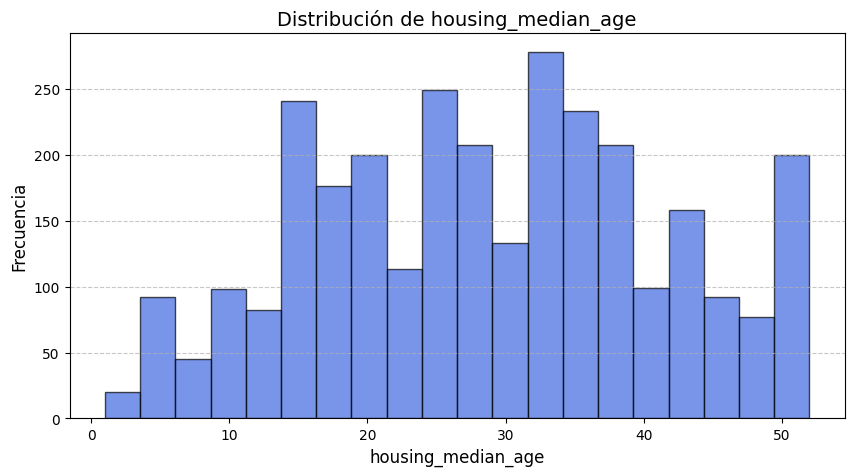
\includegraphics[width=0.8\textwidth]{housing_median_age1}
        \caption{Distribución de la Edad Mediana de las Viviendas.}
    \end{figure}

    \item \textbf{Gráfica 2:} Se puede afirmar que el promedio de edad de las viviendas es de 29 años, al igual que la mediana. Esto significa que el 50\% de las viviendas tienen menos de 29 años y el otro 50\% tienen más. En el caso de la moda, se observa que hay muchas viviendas con más de 50 años.
    \begin{figure}[H]
        \centering
        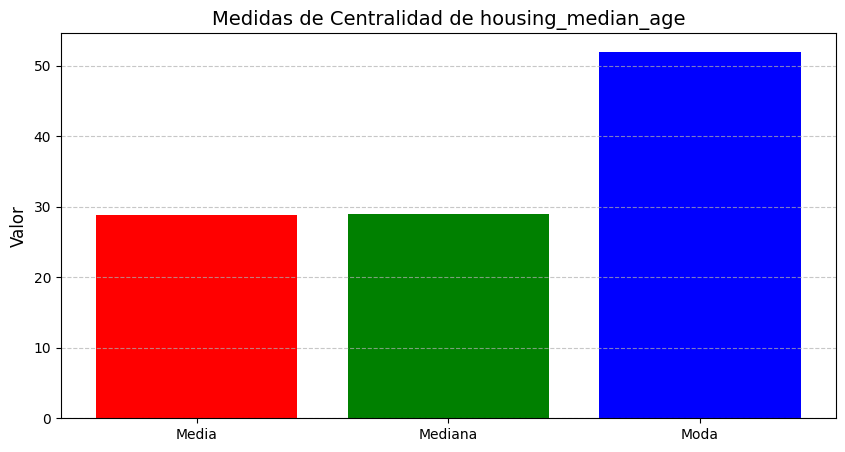
\includegraphics[width=0.8\textwidth]{housing_median_age2}
        \caption{Medidas de Centralidad de la Edad Mediana de las Viviendas.}
    \end{figure}

    \item \textbf{Gráfica 3:} Se observa que las edades de las viviendas se encuentran entre 0 y más de 50 años. El 50\% de las viviendas están representadas en la caja del diagrama, con edades que oscilan entre 18 y 36 años aproximadamente. La media está entre 28 y 29 años, lo que confirma la concentración de viviendas en ese rango.
    \begin{figure}[H]
        \centering
        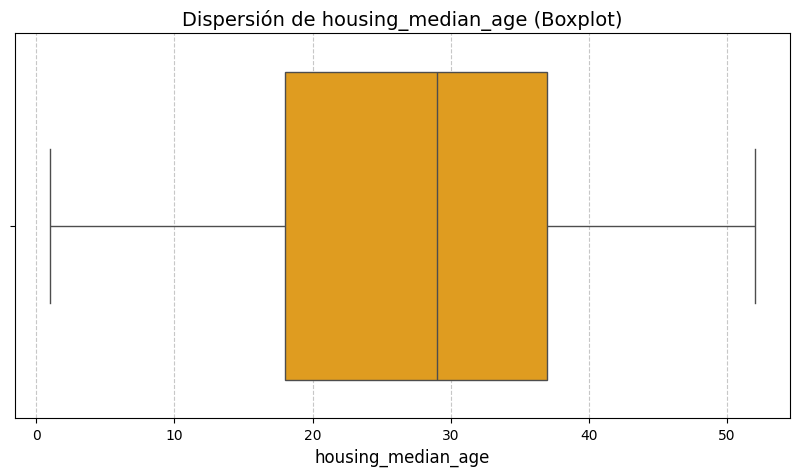
\includegraphics[width=0.8\textwidth]{housing_median_age3}
        \caption{Diagrama de Caja de la Edad Mediana de las Viviendas.}
    \end{figure}
\end{itemize}

\subsection{Total Rooms (Total de Habitaciones)}

\begin{itemize}
    \item \textbf{Gráfica 1:} La mayoría de las viviendas tienen entre 0 y 5.000 habitaciones. Sin embargo, se observa que hay algunas con hasta 25.000 habitaciones, lo que podría representar valores atípicos o errores en los datos.
    \begin{figure}[H]
        \centering
        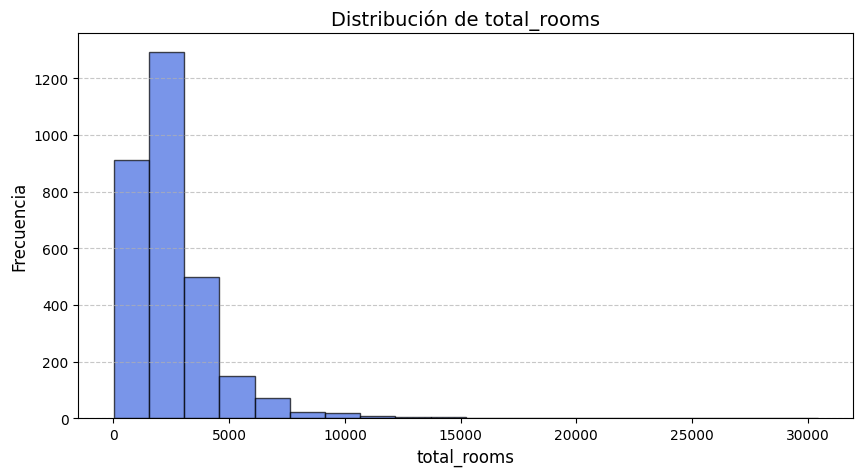
\includegraphics[width=0.8\textwidth]{Total_rooms1}
        \caption{Distribución Total de Habitaciones.}
    \end{figure}

    \item \textbf{Gráfica 2:} Se puede afirmar que el promedio de habitaciones es superior a 2.500, al igual que la mediana que está por encima de las 2.000 habitaciones. Esto significa que el 50\% de las viviendas tienen menos de 2,000 habitaciones y el otro 50\% tienen más. En el caso de la moda, se observa que hay muchas viviendas con cerca de 1,000 habitaciones.
    \begin{figure}[H]
        \centering
        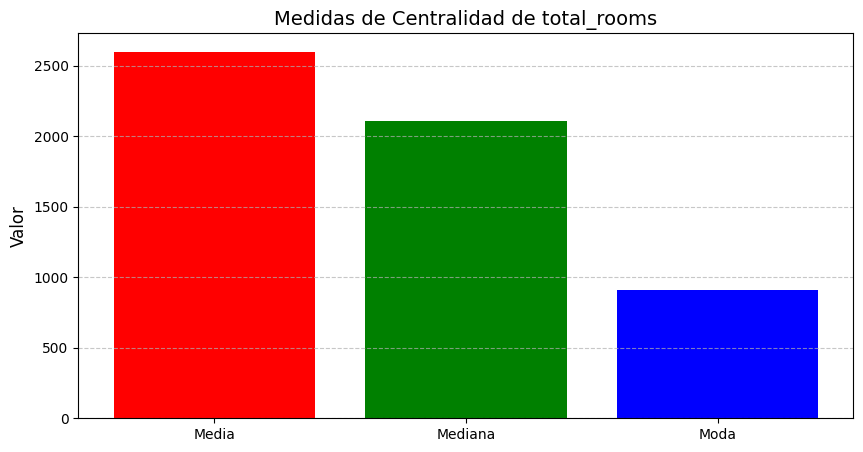
\includegraphics[width=0.8\textwidth]{Total_rooms2}
        \caption{Medidas de Centralidad de Total de Habitaciones.}
    \end{figure}

    \item \textbf{Gráfica 3:} El 50\% de las viviendas tienen entre 1.500 y 3.000 habitaciones. La media sigue siendo superior a 2500 habitaciones. Los bigotes indican que los valores típicos oscilan entre 0 y 5.100 habitaciones.
    Además, se observa una gran cantidad de valores atípicos, es decir, viviendas con cantidades de habitaciones muy alejadas de la media, que están fuera del rango del IQR.
    \begin{figure}[H]
        \centering
        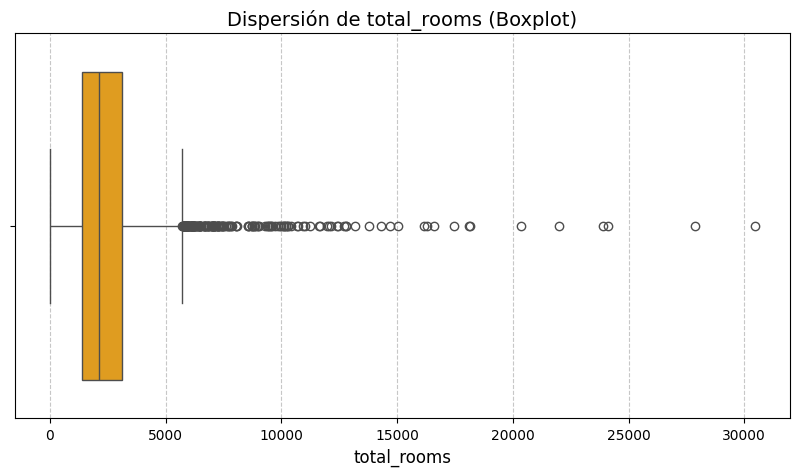
\includegraphics[width=0.8\textwidth]{Total_rooms3}
        \caption{Diagrama de Caja de Total de Habitaciones.}
    \end{figure}
\end{itemize}

\subsection{Total Bedrooms (Total de Dormitorios)}

\begin{itemize}
    \item \textbf{Gráfica 1:} El número total de dormitorios oscila entre 0 y menos de 3.000. La mayoría de las viviendas tienen entre 0 y 1.000 dormitorios, con una concentración notable alrededor de los 500 dormitorios.
    \begin{figure}[H]
        \centering
        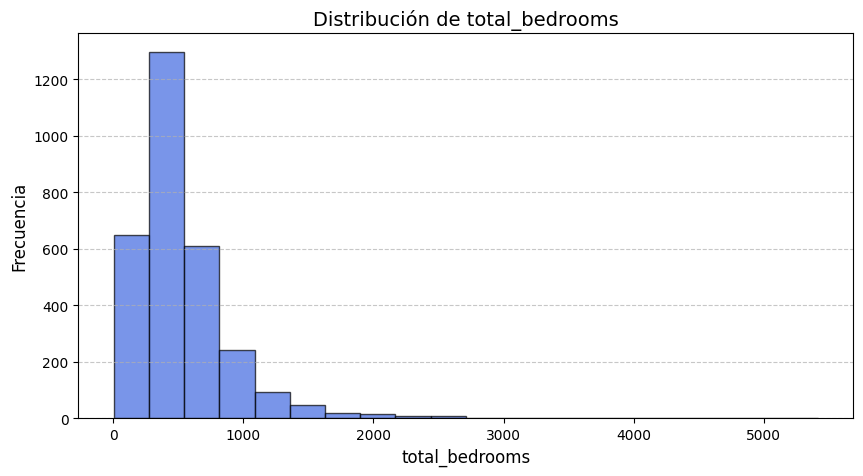
\includegraphics[width=0.8\textwidth]{Total_bedrooms1}
        \caption{Distribución Total de Dormitorios.}
    \end{figure}

    \item \textbf{Gráfica 2:} Se puede afirmar que el promedio de dormitorios es superior a 500, al igual que la mediana, que supera los 400 dormitorios. Esto significa que el 50% de las viviendas tienen menos de 400 dormitorios y el otro 50% tienen más. En el caso de la moda, se observa que hay muchas viviendas con 310 dormitorios.
    \begin{figure}[H]
        \centering
        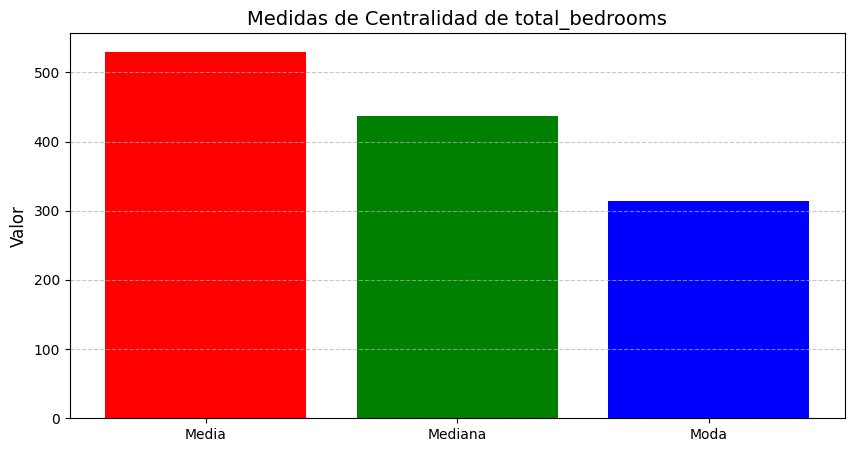
\includegraphics[width=0.8\textwidth]{Total_bedrooms2}
        \caption{Medidas de Centralidad de Total de Dormitorios.}
    \end{figure}

    \item \textbf{Gráfica 3:} El 50% de las viviendas tienen entre 400 y 500 dormitorios, los valores típicos oscilan entre 0 y 1,100 dormitorios.
    Existen muchos valores atípicos, con viviendas que tienen entre 1,100 y 2,000 dormitorios e incluso algunas con más de 5,000 dormitorios, lo que podría representar casos especiales o errores en los datos.

    \begin{figure}[H]
        \centering
        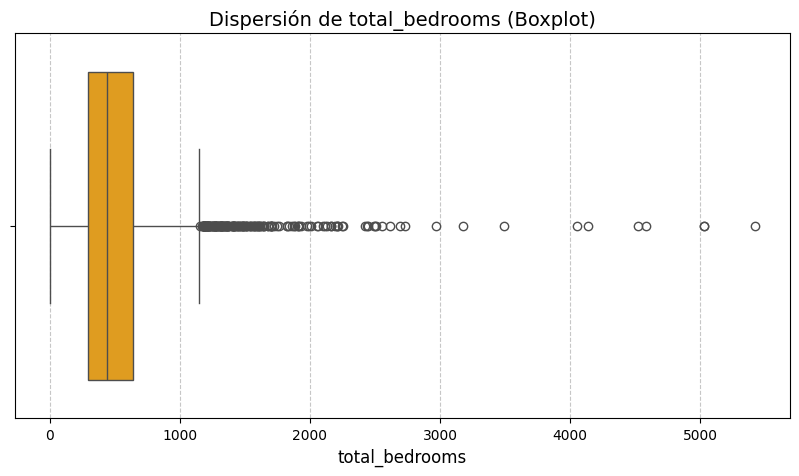
\includegraphics[width=0.8\textwidth]{Total_bedrooms3}
        \caption{Diagrama de Caja de Total de Dormitorios.}
    \end{figure}
\end{itemize} 

\subsection{Population (Población en las zonas)}

\begin{itemize}
    \item \textbf{Gráfica 1:} La mayoría de las zonas tienen una población entre 0 y 2,000 personas. Sin embargo, hay valores que se extienden hasta 12,000 habitantes, lo que puede indicar desde ya la presencia de valores atípicos.
    \begin{figure}[H]
        \centering
        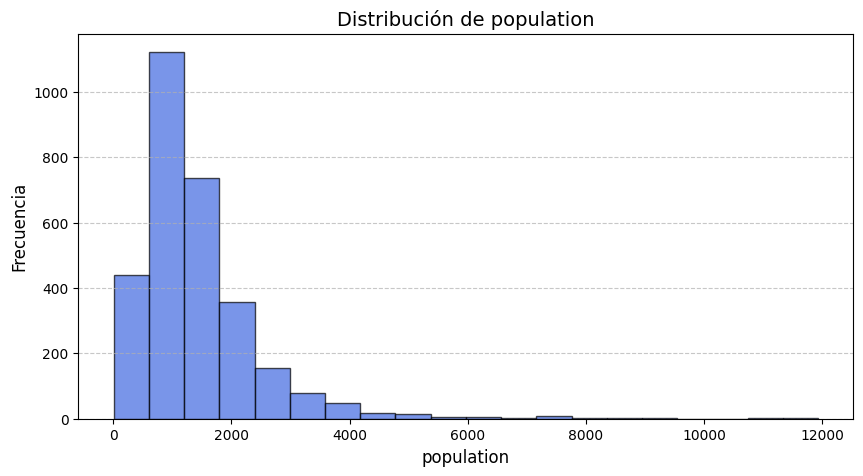
\includegraphics[width=0.8\textwidth]{population1}
        \caption{Distribución de la Población en las zonas.}
    \end{figure}

    \item \textbf{Gráfica 2:} Se puede afirmar que el promedio de población es de 1.400 personas, al igual que la mediana, que es de aproximadamente 1.200 personas. Esto significa que el 50\% de las zonas tienen menos de 1.200 habitantes y el otro 50\% tienen más. En el caso de la moda, se observa que muchas zonas tienen alrededor de 850 habitantes.
    \begin{figure}[H]
        \centering
        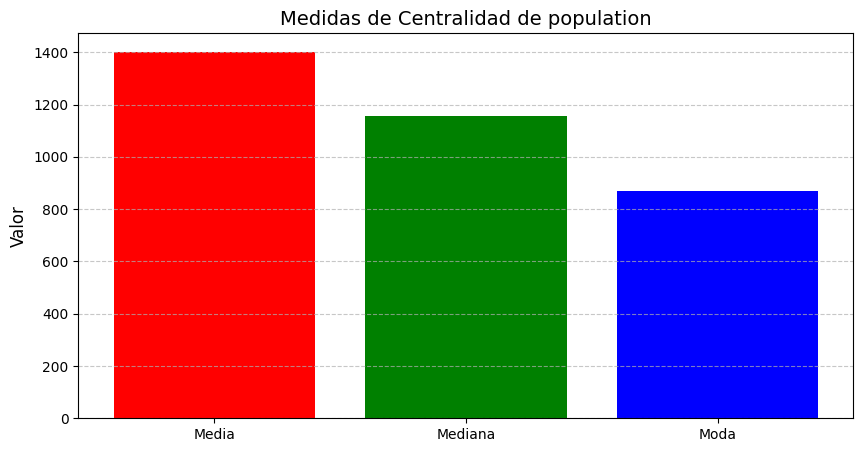
\includegraphics[width=0.8\textwidth]{population2}
        \caption{Medidas de Centralidad de la Población en las zonas.}
    \end{figure}

    \item \textbf{Gráfica 3:} Los valores típicos de la población oscilan entre 0 y 3.200 habitantes, el 50\% de las zonas tienen una población entre 1.000 y casi 2.000 personas. Se observa una gran cantidad de valores atípicos en poblaciones superiores a 3.200 habitantes.
    \begin{figure}[H]
        \centering
        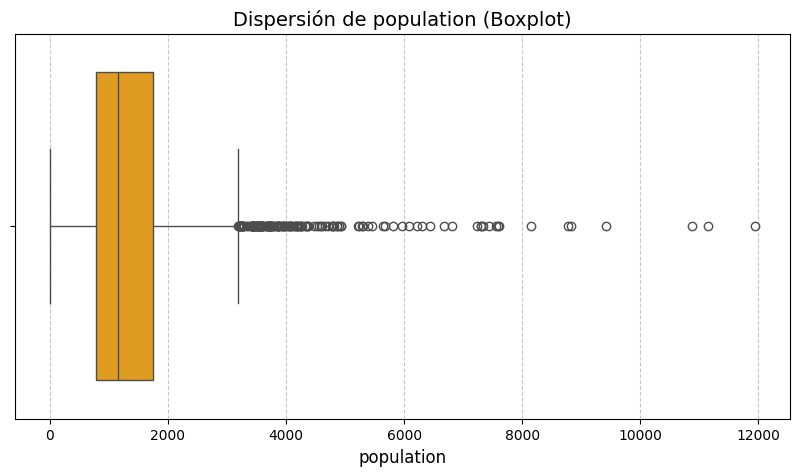
\includegraphics[width=0.8\textwidth]{population3}
        \caption{Diagrama de Caja de la Población en las zonas.}
    \end{figure}
\end{itemize}

\subsection{Households (Número de Hogares por Zona)}

\begin{itemize}
    \item \textbf{Gráfica 1:} La mayoría de las zonas tienen pocos hogares, más de 1.200 zonas cuentan con apenas 500 hogares. Y que solo algunas zonas superan los 3.000 hogares.
    \begin{figure}[H]
        \centering
        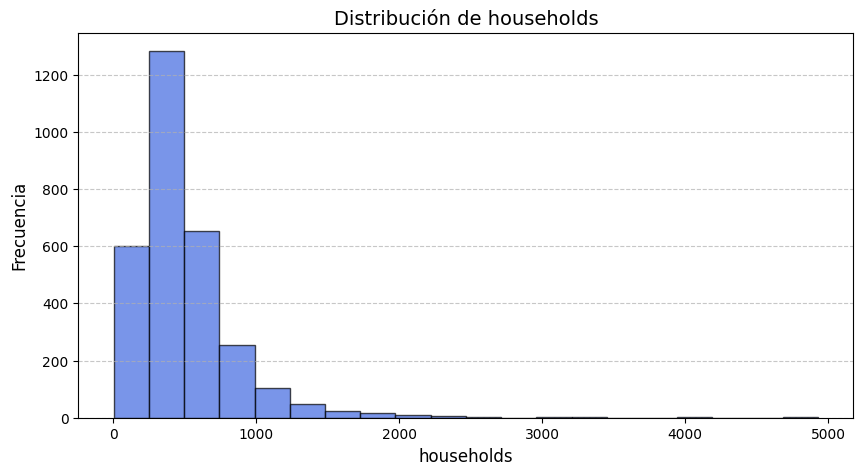
\includegraphics[width=0.8\textwidth]{households1}
        \caption{Distribución de Número de Hogares por Zona.}
    \end{figure}

    \item \textbf{Gráfica 2:} Se puede afirmar que el promedio de hogares es menor a 500, la mediana por su parte está por encima de 400 hogares. Esto significa que el 50\% de las zonas tienen menos de 400 hogares y el otro 50\% tienen más. En el caso de la moda, se observa que muchas zonas tienen cerca de 380 hogares.
    \begin{figure}[H]
        \centering
        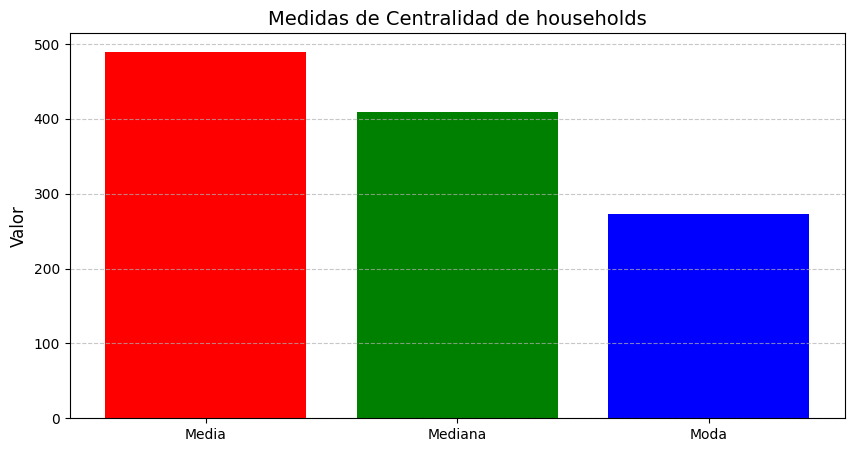
\includegraphics[width=0.8\textwidth]{households2}
        \caption{Medidas de Centralidad de Número de Hogares por Zona.}
    \end{figure}

    \item \textbf{Gráfica 3:} Los valores típicos oscilan entre 0 y un poco más de 10000 hogares. Muchas zonas tienen menos de 10000 hogares, pero hay algunas con más de 2.000 o incluso 50000 hogares, lo que las convierte en valores atípicos.
    \begin{figure}[H]
        \centering
        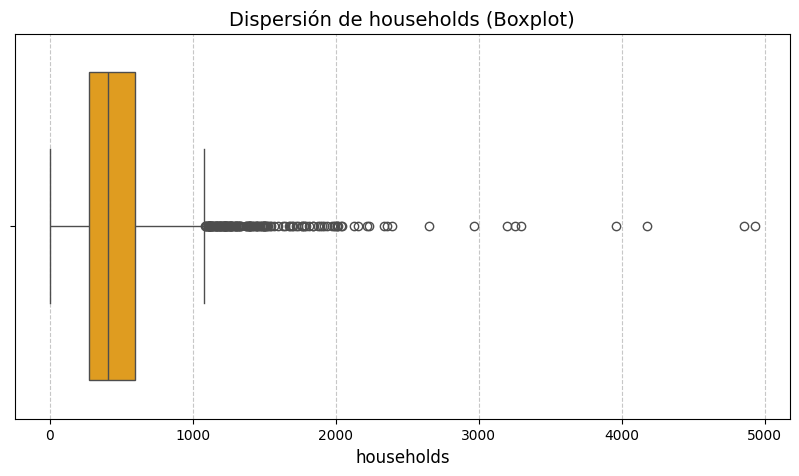
\includegraphics[width=0.8\textwidth]{households3}
        \caption{Diagrama de Caja de Número de Hogares por Zona.}
    \end{figure}
\end{itemize}



\subsection{Median Income (Ingreso Mediano por Zona)}

\begin{itemize}
    \item \textbf{Gráfica 1:} La mayoría de las zonas tienen ingresos medianos entre 2 y 5, pero existen algunas con ingresos significativamente más altos.
    \begin{figure}[H]
        \centering
        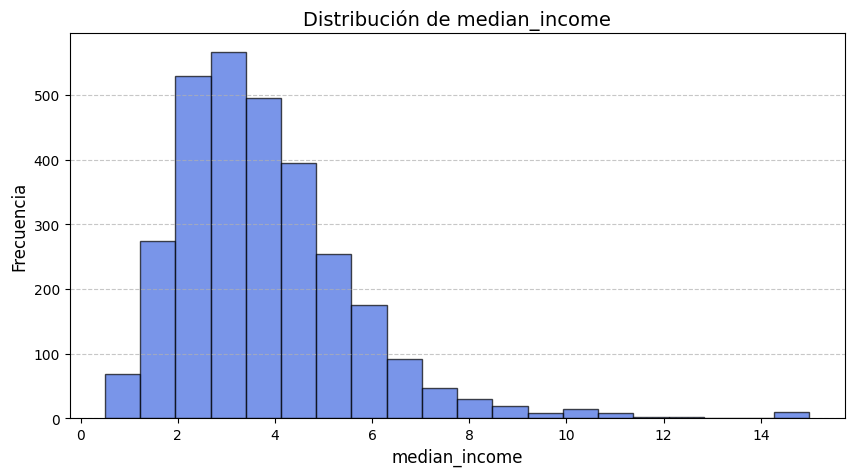
\includegraphics[width=0.8\textwidth]{median_income1}
        \caption{Distribución de Ingreso Mediano por Zona.}
    \end{figure}

    \item \textbf{Gráfica 2:} Se puede afirmar que el promedio de ingreso mediano es aproximadamente 4, al igual que la mediana. Esto significa que el 50% de las zonas tienen un ingreso menor a 4 y el otro 50% tienen ingreso superior a ese valor. En el caso de la moda, se observa que muchas zonas tienen un ingreso de 15.
    \begin{figure}[H]
        \centering
        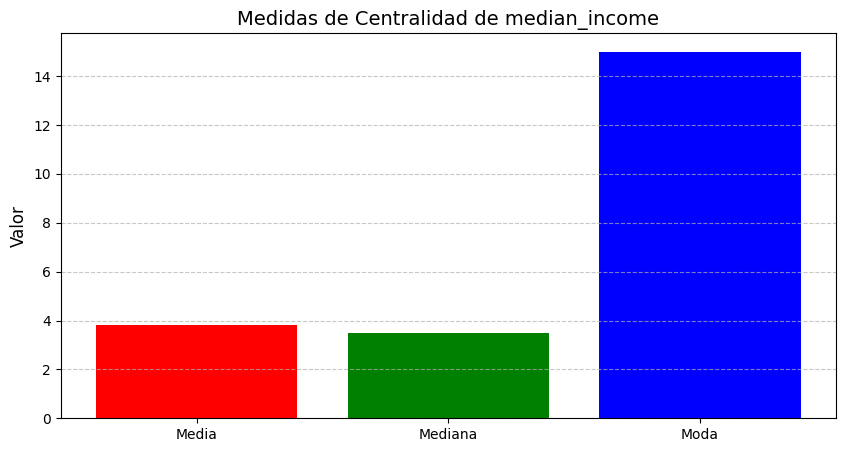
\includegraphics[width=0.8\textwidth]{median_income2}
        \caption{Medidas de Centralidad de Ingreso Mediano por Zona.}
    \end{figure}

    \item \textbf{Gráfica 3:} : Los valores típicos oscilan entre 0 y menos de 8, el 50% de las zonas tienen ingresos entre 3 y menos de 5.
    \begin{figure}[H]
        \centering
        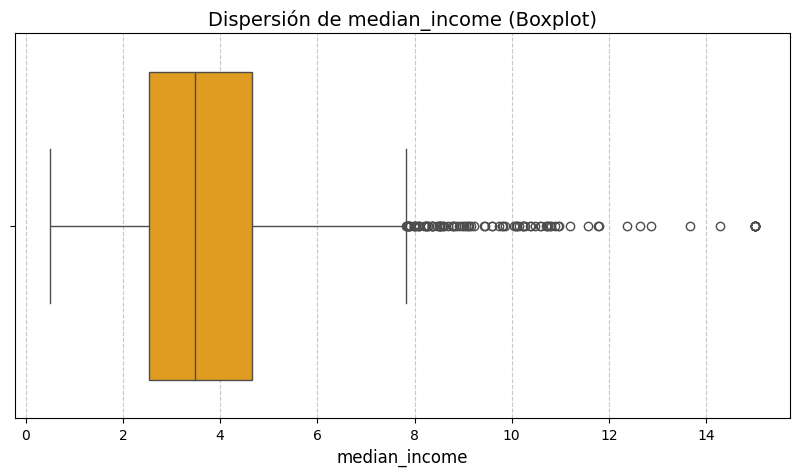
\includegraphics[width=0.8\textwidth]{median_income3}
        \caption{Diagrama de Caja de Ingreso Mediano por Zona.}
    \end{figure}
\end{itemize}

\subsection{Median House Value (Valor Mediano de las Viviendas)}

\begin{itemize}
    \item \textbf{Gráfica 1:} La mayoría de las zonas tienen ingresos medianos entre 2 y 5, pero existen algunas con ingresos significativamente más altos.
    \begin{figure}[H]
        \centering
        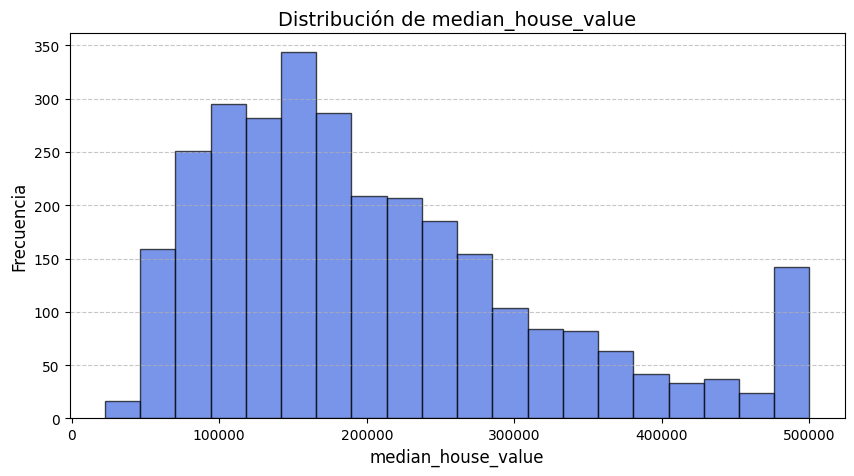
\includegraphics[width=0.8\textwidth]{median_house_value1}
        \caption{Distribución de Valor Mediano de las Viviendas.}
    \end{figure}

    \item \textbf{Gráfica 2:} La mayoría de las viviendas tienen valores entre 100.000 y 200.000 dólares.
A medida que aumenta el valor de las viviendas, la frecuencia disminuye, hasta llegar a 5000000, donde hay un aumento significativo en este valor.

    \begin{figure}[H]
        \centering
        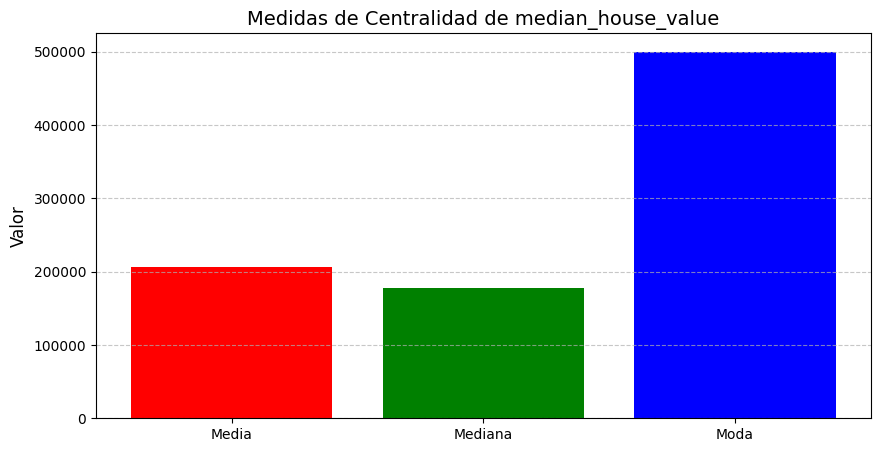
\includegraphics[width=0.8\textwidth]{median_house_value2}
        \caption{Medidas de Centralidad de Valor Mediano de las Viviendas.}
    \end{figure}

    \item \textbf{Gráfica 3:} : : La mayoría de las viviendas tienen valores entre 1000.000 y 300.0000 dólares, que viviendas con un valor de 500.000 dólares se consideran valores atípicos según los valores y el calco del IQR.
    \begin{figure}[H]
        \centering
        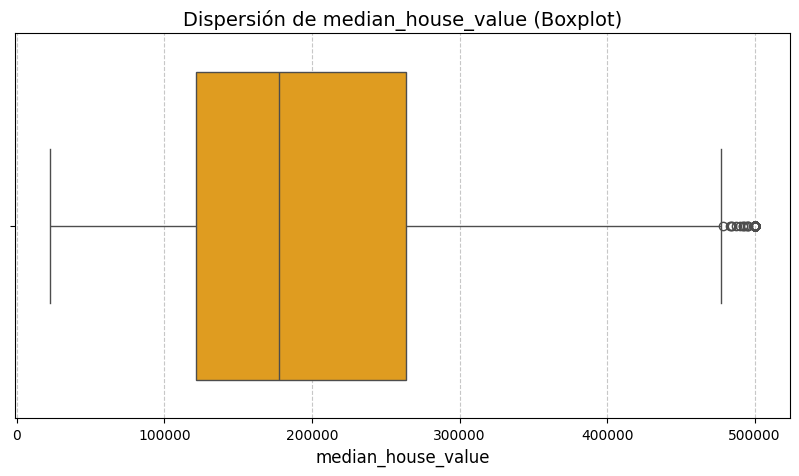
\includegraphics[width=0.8\textwidth]{median_house_value3}
        \caption{Diagrama de Caja de Valor Mediano de las Viviendas.}
    \end{figure}
\end{itemize}


\section{Análisis Multivariado}

\subsection{Análisis de la Matriz de Correlación}

total\_rooms y total\_bedrooms están altamente correlacionados (0.94), lo que nos dice que ambas proporcionan información similar, que median\_house\_value tiene una relación muy débil con ambas variables, lo que sugiere que el número de habitaciones o dormitorios no es un factor clave para determinar el precio de la vivienda.

\begin{figure}[H]
    \centering
    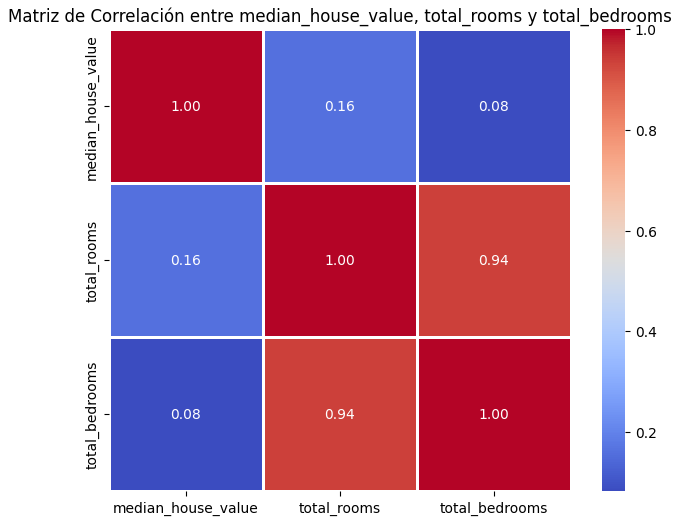
\includegraphics[width=0.8\textwidth]{multivariado1.png} % Cambia el nombre y la ruta del archivo de la imagen si es necesario
    \caption{Matriz de Correlación entre total\_rooms, total\_bedrooms y median\_house\_value.}
\end{figure}



\subsection{Relación entre Total de Habitaciones y Valor de la Vivienda}

El gráfico muestra que no hay una relación entre el número de habitaciones y el valor de la vivienda, ya que los datos se encuentran dispersos y no hay una tendencia definida. La mayoría de las viviendas tienen menos de 5.000 habitaciones, pero incluso entre ellas, el valor de las casas varía ampliamente. 

\begin{figure}[H]
    \centering
    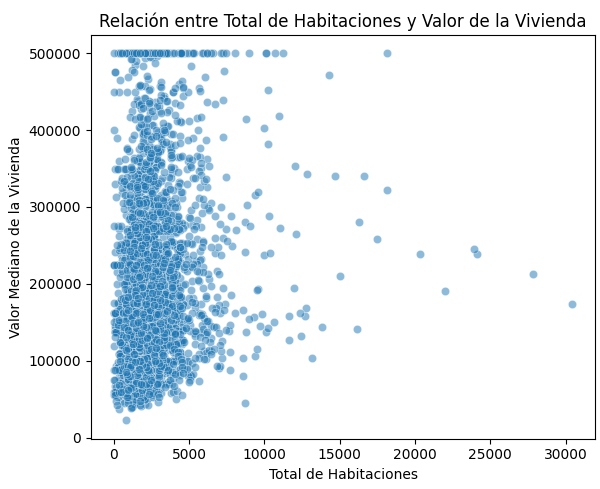
\includegraphics[width=0.8\textwidth]{multivariado2.png} % Cambia el nombre y la ruta del archivo de la imagen si es necesario
    \caption{Relación entre Total de Habitaciones y Valor de la Vivienda.}
\end{figure}

\subsection{Relación entre Total de Habitaciones y Total de Dormitorios}

Este gráfico nos muestra una fuerte correlación positiva entre el número total de habitaciones y el número total de dormitorios, con una tendencia lineal. A medida que aumenta la cantidad de habitaciones, también lo hace la cantidad de dormitorios, lo que tiene sentido ya que una mayor cantidad de habitaciones en una vivienda generalmente implica más dormitorios.  

\begin{figure}[H]
    \centering
    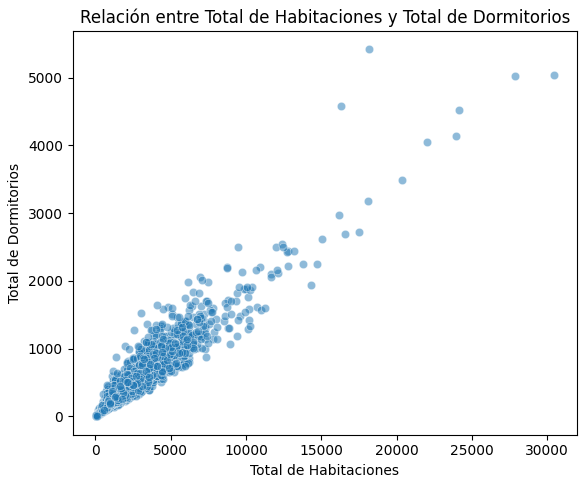
\includegraphics[width=0.8\textwidth]{multivariado3.png} % Cambia el nombre y la ruta del archivo de la imagen si es necesario
    \caption{Relación entre Total de Habitaciones y Total de Dormitorio.}
\end{figure}


\section{Conclusiones}
El análisis realizado muestra que ni el número de habitaciones ni el número de dormitorios tienen una fuerte influencia en el valor de la vivienda en California. Sin embargo, estas dos variables están altamente correlacionadas entre sí, lo que indica que una de ellas podría ser eliminada sin perder información significativa en un análisis predictivo. Otras variables, como la ubicación o el ingreso mediano de la zona, podrían ser factores más determinantes en el valor de las viviendas. Estos resultados sugieren que un estudio más profundo, incluyendo otras variables, podría proporcionar una mejor comprensión de los factores que afectan los precios de las viviendas.

\section{Referencias}
\begin{itemize}
    \item \url{https://www.youtube.com/watch?v=7GzcFTWPAds} - Análisis multivariable, ¿de qué se trata? Básico y simplificado.
    \item \url{https://www.youtube.com/watch?v=RzPzqvkTZRU&t=387s} - Análisis univariable, ¿de qué se trata? Básico y simplificado.
\end{itemize}

\end{document}